%!TEX root = ../main.tex
\appendix
\addchap{Annexes}

\renewcommand{\thesection}{\Alph{section}}
\label{appendix}

% create a table of appendices here manually like this:
\contentsline{section}{\numberline{A}Cycle de vie SecurityByDesign}
    {\pageref{appendix:securitybydesign}}{appendix:securitybydesign}
\contentsline{section}{\numberline{B}Processus fils de l’audit de sécurité d’une application : actions techniques}
    {\pageref{appendix:subprocessaudit}}{appendix:subprocessaudit}
\contentsline{section}{\numberline{C}Processus de l'audit de sécurité d'une application}
    {\pageref{appendix:processaudit}}{appendix:processaudit}
\contentsline{section}{\numberline{D}Rétroplanning du projet}
    {\pageref{appendix:retroplan}}{appendix:retroplan}    

\newpage

%!TEX root = ../main.tex
\section{Cycle de vie SecurityByDesign}
\label{appendix:securitybydesign}
\vspace{2em}
\centering
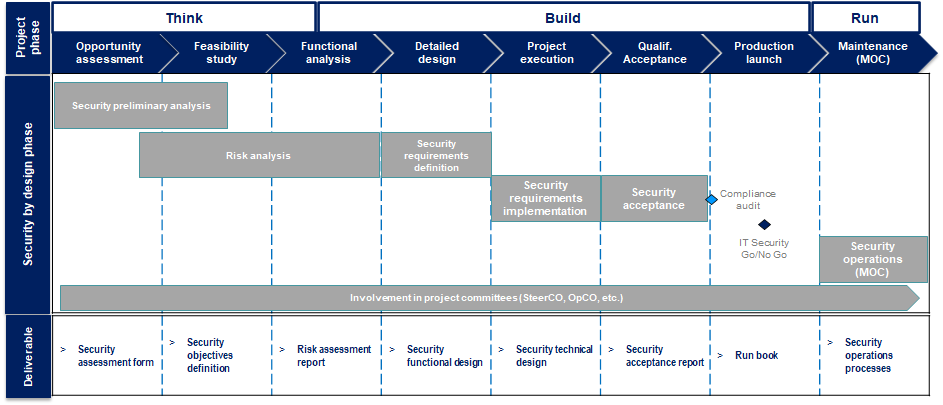
\includegraphics[width=0.8\textheight, angle=90,origin=c]{resources/img/security_by_design.png}
%!TEX root = ../main.tex
\section{Processus fils de l’audit de sécurité d’une application : actions techniques}
\label{appendix:subprocessaudit}
\vspace{2em}
\centering
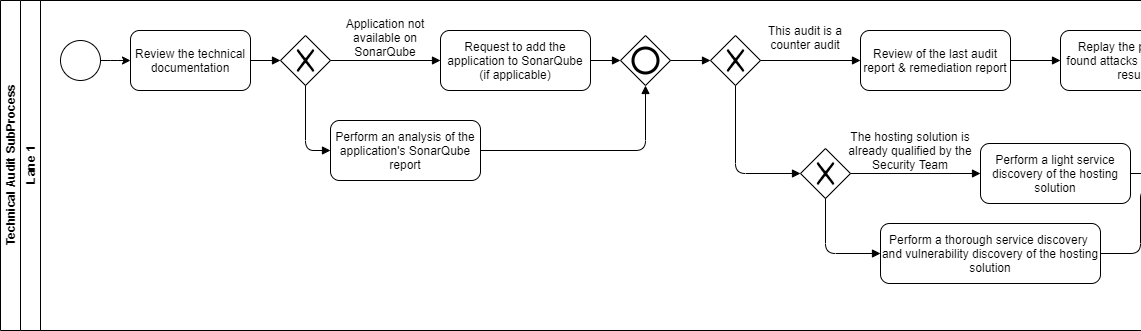
\includegraphics[width=\textwidth]{resources/img/technical_audit_subprocess_pt1.png}
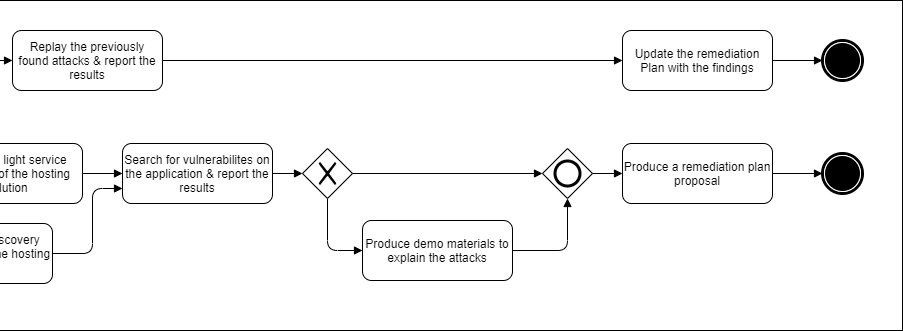
\includegraphics[width=\textwidth]{resources/img/technical_audit_subprocess_pt2.png}
%!TEX root = ../main.tex
\section{Processus de l'audit de sécurité d'une application}
\label{appendix:processaudit}
\vspace{2em}
\centering
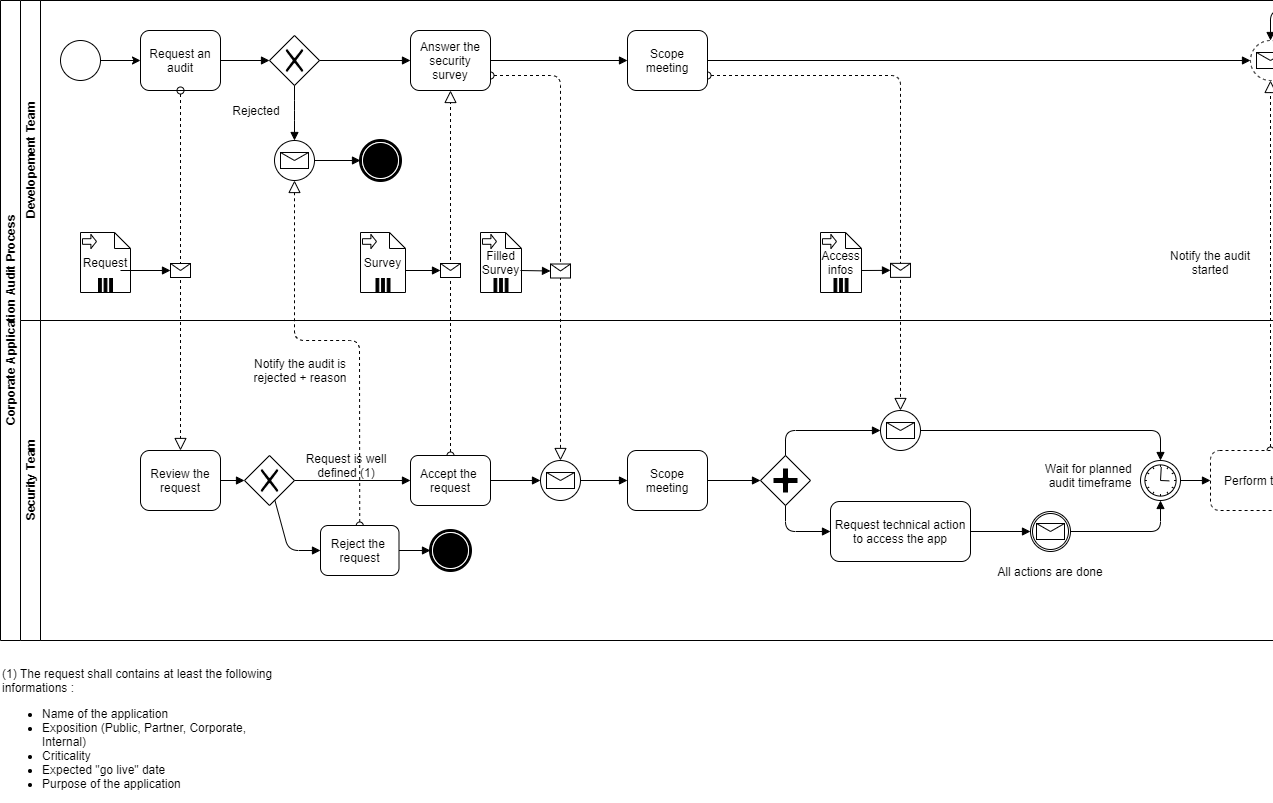
\includegraphics[width=\textwidth]{resources/img/process_audit_pt1.png}
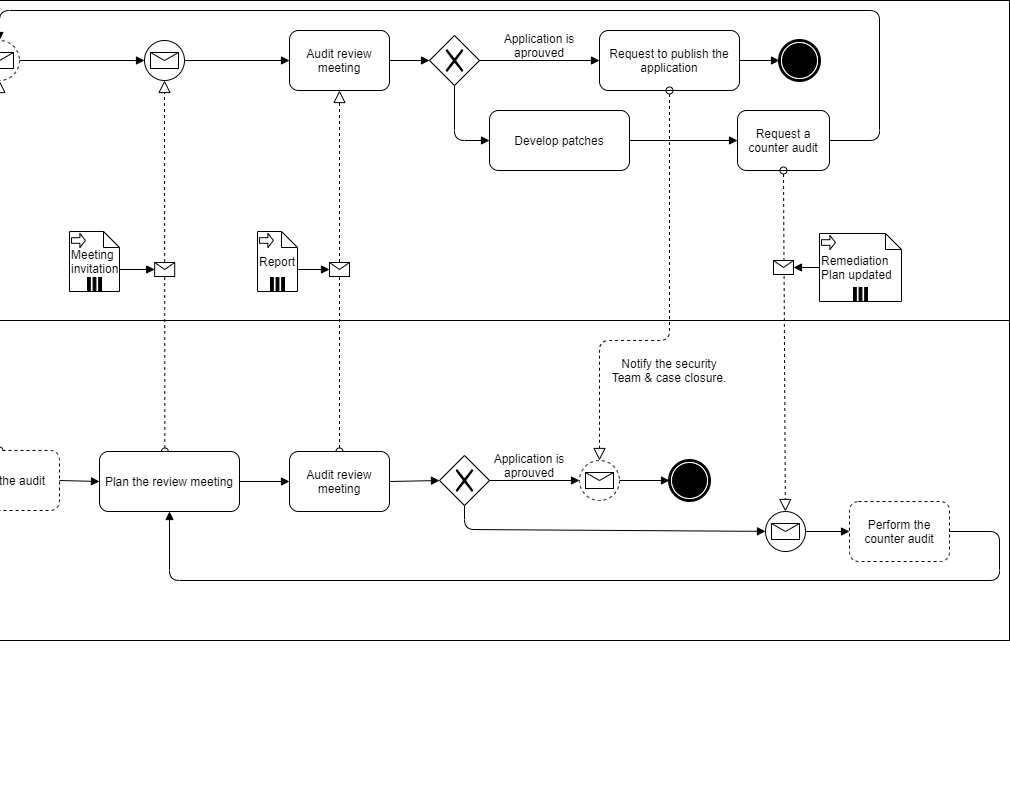
\includegraphics[width=\textwidth]{resources/img/process_audit_pt2.png}
%!TEX root = ../main.tex
\section{Rétroplanning du projet}
\label{appendix:retroplan}
\vspace{2em}
\centering
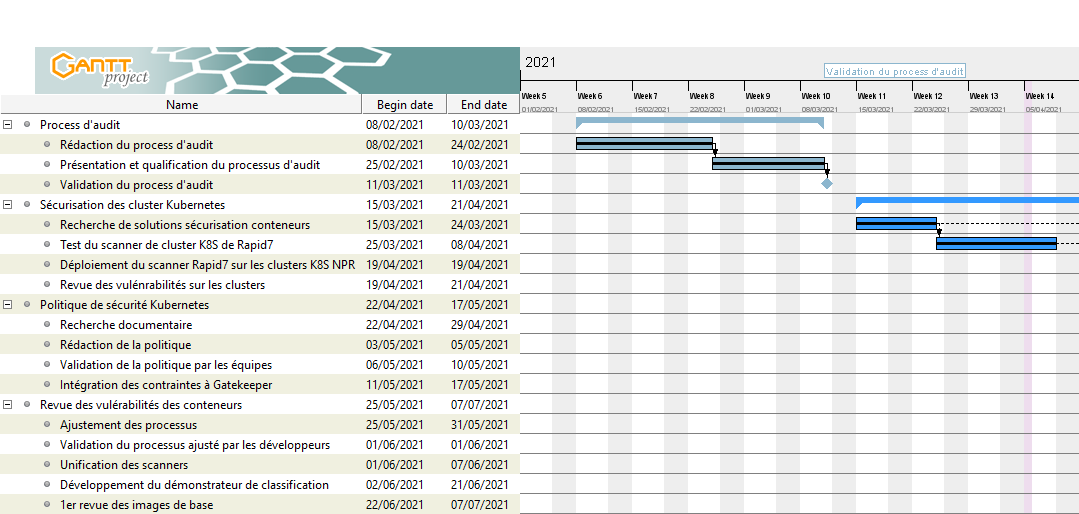
\includegraphics[width=\textwidth]{resources/img/retroplanning_pt1.png}
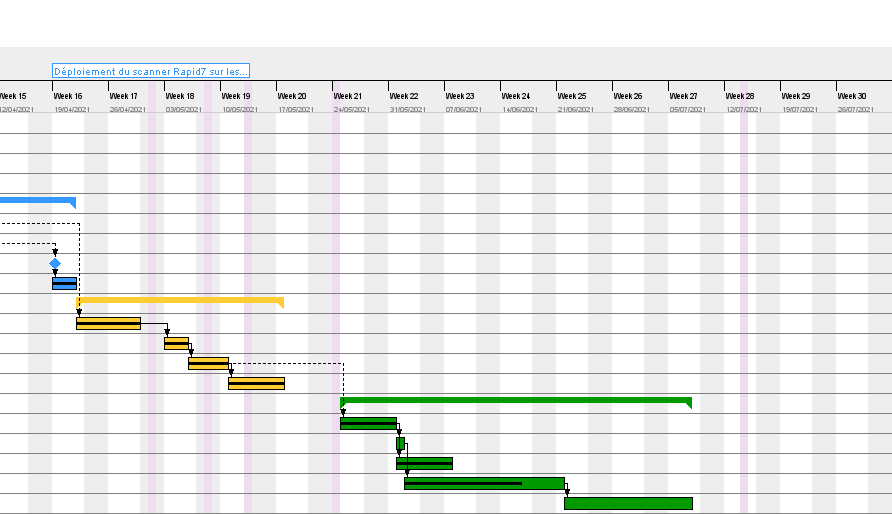
\includegraphics[width=\textwidth]{resources/img/retroplanning_pt2.png}


% input the appendix files here like this:
%  \input{appendix/appendix1.tex}
%  \newpage
